%%%%%%%%%%%%%%%%%%%%%%%%%%%%%%%%%%%%%%%%%
% Revista Difu100cia
%%%%%%%%%%%%%%%%%%%%%%%%%%%%%%%%%%%%%%%%%
\documentclass[12pt]{difu100cia} % clase difu100cia

%----------------------------------------------------------------------------------------
%	PAQUETES ADICIONALES
%----------------------------------------------------------------------------------------


%----------------------------------------------------------------------------------------
%	DECLARACION DE COMANDOS
%----------------------------------------------------------------------------------------


%----------------------------------------------------------------------------------------
%	INFORMACION DEL ARTICULO
%----------------------------------------------------------------------------------------

\title{Template for article submission to $\boldsymbol{\mathcal{DIFU}_{100}ci@}$ magazine} % Titulo del articulo en ingles
\subtitle{Plantilla para el envío de artículos a la revista $\boldsymbol{\mathcal{DIFU}_{100}ci@}$} % Titulo del articulo en espanol
% Autores
%\author[1]{\authorstyle{Autor 1}\thanks{Corresponding author}}
\author[1]{\authorstyle{Autor 1}\thanks{Autor de correspondencia}}
\author[1]{\authorstyle{Autor 2}}
\author[2]{\authorstyle{Autor 3}}
\affil[1]{\institution{Instituto 1, Area 1, \authorcr Departamento 1, \authorcr Calle, Número, Colonia, Ciudad, Estado, País, CP. \authorcr \{autor1,autor2\}@dominio.com }}
\affil[2]{\institution{Instituto 2, Area 2, \authorcr Departamento 2, \authorcr Calle, Número, Colonia, Ciudad, Estado, País, CP. \authorcr autor3@dominio.com }}

%----------------------------------------------------------------------------------------
%   Fecha de publicación
%----------------------------------------------------------------------------------------

\publishrange{xxxx - xxxx xxxx}
\volume{XX}
\num{X}
\published{XX de xxxx de xxxx}

%----------------------------------------------------------------------------------------

\begin{document}
\thispagestyle{firstpage} % Aplica el estilo en la primera pagina sin cabeceras y pie de pagina
\pagestyle{fancy}
%----------------------------------------------------------------------------------------
%	RESUMEN
%----------------------------------------------------------------------------------------
\twocolumn[\begin{@twocolumnfalse}
\maketitle % Imprime el titulo
\selectlanguage{english} 
\begin{abstract}
The summary is a single paragraph with a maximum of 8 lines, in which the work carried out in the article will be explained in a clear and condensed manner.
\end{abstract}

\keywords{keyword 1, keyword 2, keyword 3}

\selectlanguage{spanish} 
\begin{abstract}
El resumen debe ser un párrafo de un máximo de 8 renglones, en ella se explicará de forma clara y condensada el trabajo realizado en el artículo.
\end{abstract}

\keywords{Palabra clave 1, Palabra clave 2, Palabra clave 3}
\vspace{3em}
\end{@twocolumnfalse}]
\saythanks

%----------------------------------------------------------------------------------------
%	ARTICULO
%----------------------------------------------------------------------------------------

%\selectlanguage{english} % Selecciona ingles como idioma del texto del ariculo

\section{Introducción}
\lettrinesection{E}n la revista $\boldsymbol{\mathcal{DIFU}_{100}ci@}$ se puede someter tanto en español como en inglés, para los artículos escritos en inglés se debe de descomentar la línea 

\begin{lstlisting}[basicstyle=\small]
    \selectlanguage{english} 
\end{lstlisting}

Esto permitirá que los pie de figura y los títulos de las tablas aparezcan en inglés de forma automática.

\section{Secciones y subsecciones}

Las secciones se realizan a través del comando 

\begin{lstlisting}[basicstyle=\small]
    \section{Seccion} 
\end{lstlisting}

Las subsecciones 

\begin{lstlisting}[basicstyle=\small]
    \subsection{Subseccion} 
\end{lstlisting}

Para un nivel mas de indización no se recomienda el comando

\begin{lstlisting}[basicstyle=\small]
    \subsubsection{Subsubseccion} 
\end{lstlisting}

En su lugar se recomienda solo el uso de negritas

\begin{lstlisting}[basicstyle=\small]
    \noindent
    \newline
    \textbf{Subsubseccion}
    \newline
\end{lstlisting}

\section{Figuras}

La clase de \textit{difu100cia.cls} busca de forma automática las figuras localizadas en las carpetas \textit{Figuras} y \textit{Figures}, estas pueden ser jpg, png, bmp y eps.

Para agregar una figura en una sola columna se utiliza el siguiente código:

\begin{lstlisting}[basicstyle=\small]
    \begin{figure}[!ht]
	\centering
	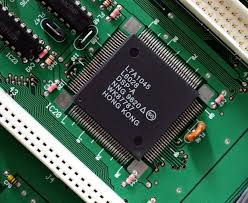
\includegraphics[width=\linewidth]{fig01}
	\caption{Pie de Figura 01}
	\label{fig:01}
\end{figure}
\end{lstlisting}

Para que la figura utilice dos columnas 

\begin{lstlisting}[basicstyle=\small]
    \begin{figure*}[!ht]
	\centering
	
\includegraphics[width=\linewidth]{fig02}
	\caption{Pie de Figura 02}
	\label{Pie de Figura 02}
\end{figure*}
\end{lstlisting}

Para agrupar varias figuras se utiliza el comando 

\begin{lstlisting}[basicstyle=\small]
    \begin{figure}
     \centering
     \begin{subfigure}[b]{0.45\textwidth}
         \centering
         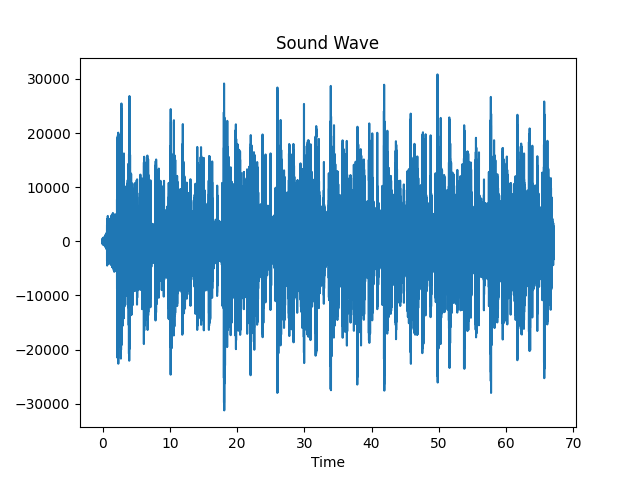
\includegraphics[width=\textwidth]{fig03a.png}
         \caption{Pie de Figura 03a}
         \label{fig:03a}
     \end{subfigure}
     \hfill
     \begin{subfigure}[b]{0.45\textwidth}
         \centering
         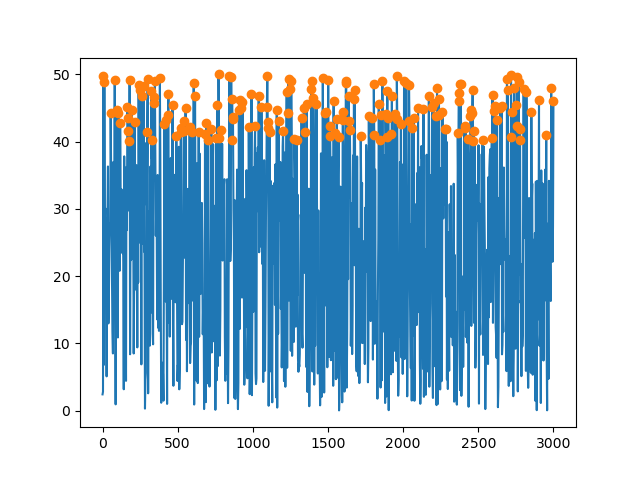
\includegraphics[width=\textwidth]{fig03b.png}
         \caption{Pie de Figura 03b}
         \label{fig:03b}
     \end{subfigure}
     \hfill
     \begin{subfigure}[b]{0.45\textwidth}
         \centering
         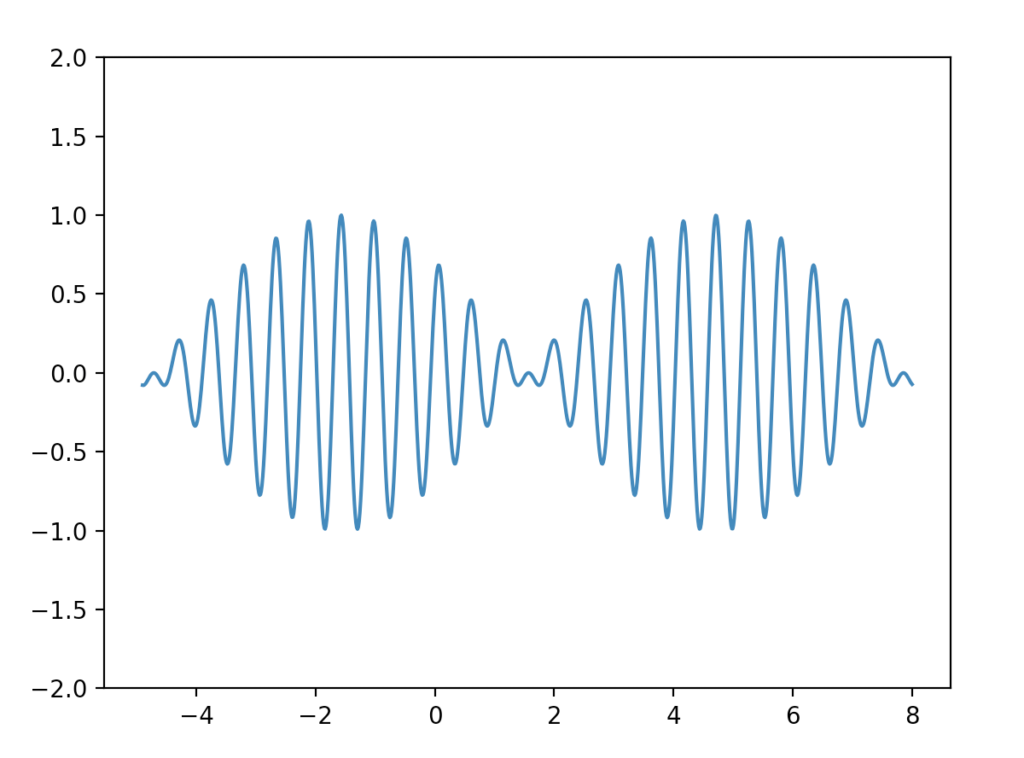
\includegraphics[width=\textwidth]{fig03c.png}
         \caption{Pie de Figura 03c}
         \label{fig:03c}
     \end{subfigure}
        \caption{Pie de Figura 03}
        \label{fig:03}
\end{figure}
\end{lstlisting}

\section{Tablas}

Las tablas se conforman solamente de tres líneas horizontales, ninguna vertical

\begin{lstlisting}[basicstyle=\small]
\begin{table}[htb!]
    \centering
    \caption{Titulo de la tabla} 
    \begin{tabular}{cc} 
        \toprule
         Tap   & Coeficiente \\ 
         \midrule
         h[-2]=h[2] & -0.09972695 \\
         h[-1]=h[1] & 0.59466396 \\
        \bottomrule
        \end{tabular}
    \label{tab:01}
    \end{table}
\end{lstlisting}

\begin{lstlisting}[basicstyle=\small]
\begin{table*}[htb!]
    \centering
    \caption{Titulo de la tabla} 
    \begin{tabular}{cc} 
        \toprule
         Tap   & Coeficiente \\ 
         \midrule
         h[-2]=h[2] & -0.09972695 \\
         h[-1]=h[1] & 0.59466396 \\
        \bottomrule
        \end{tabular}
    \label{tab:01}
    \end{table*}
\end{lstlisting}

\begin{lstlisting}
    \begin{table*}[htb!]
    \centering
    \begin{threeparttable}
    \small
    \caption{Cuadro elaborado a partir de varias publicaciones internacionales, principalmente Climate Change 1994, Intergovernmental Panel on Climate Change \cite{_instituto}}
    \begin{tabular}{m{3em}m{5em}m{7em}m{7em}m{2em}m{2em}m{2em}m{6em}m{5em}}
        \toprule
         Gas & Principales fuentes & Concentraciones preindustriales & Concentraciones actuales & \multicolumn{3}{m{9em}}{Potenciales de calentamiento global} & Crecimiento (ritmo anual) & Vida atmosferica \\
         & & & & 20 & 100 & 500 & & \\
         \midrule
         Bioxido de carbono $CO_2$* & Quema de combustible fosiles, produccion de cemento, etc. & 280 & 350 & 1 & 1 & 1 & 1.6 & 50*200 \\
         Metano $CH_4$* & Cultivo de arroz, rellenos sanitarios, ganaderia, etc. & 0.8 & 1.7 & 62 & 24.5 & 75 & 0.02 & 10 \\
         Oxido nitroso $ N_20$* & Agricultura (pastoreo en regiones tropicales),  quema de biomasa, etc. & 288 & 310 & 290 & 320 & 180 & 0.8 & 150 \\
         \bottomrule
    \end{tabular}
    \begin{tablenotes}
        \item [*]	Partes por millon
        \item [**]	Partes por mil millones
    \end{tablenotes}
    \end{threeparttable}
    \label{tab:08}
\end{table*}

\end{lstlisting}

Finalmente, las referencias se deben de agregar en el archivo referencias.bib en formato bib. 

\begin{lstlisting}
@article{wyglinski2016revolutionizing,
  title={Revolutionizing software defined radio: case studies in hardware, software, and education},
  author={Wyglinski, Alexander M and Orofino, Don P and Ettus, Matthew N and Rondeau, Thomas W},
  journal={IEEE Communications magazine},
  volume={54},
  number={1},
  pages={68--75},
  year={2016},
  publisher={IEEE}
}
\end{lstlisting}
%----------------------------------------------------------------------------------------
%	REFERENCIAS
%----------------------------------------------------------------------------------------

% Las referencias se deben de agregar en el archivo referencias.bib en formato bib. 

\printbibliography

%----------------------------------------------------------------------------------------

\end{document}
